\documentclass[aspectratio=169]{beamer}
\usetheme{boxes}
\setbeamertemplate{navigation symbols}{}
\setbeamertemplate{itemize items}[circle]
\usepackage{fontspec}
\usepackage{graphics}
\usepackage{graphicx}
\usepackage{hyperref}
\usepackage{multicol}
\usepackage{tikz}
\usepackage{xcolor}

\setmainfont{Jost}
\setsansfont{Jost}
\setmonofont{Inconsolata}

\newcommand{\btVFill}{\vskip0pt plus 1filll}
\newcommand{\q}[1]{\mathsf{#1}}

\definecolor{cb1}{RGB}{230, 159, 0}
\definecolor{cb2}{RGB}{86, 180, 233}
\definecolor{cb3}{RGB}{0, 158, 115}


\tikzset{
  invisible/.style={opacity=0},
  visible on/.style={alt={#1{}{invisible}}},
  alt/.code args={<#1>#2#3}{%
    \alt<#1>{\pgfkeysalso{#2}}{\pgfkeysalso{#3}} % \pgfkeysalso doesn't change the path
  },
}

\begin{document}

\begin{frame}
  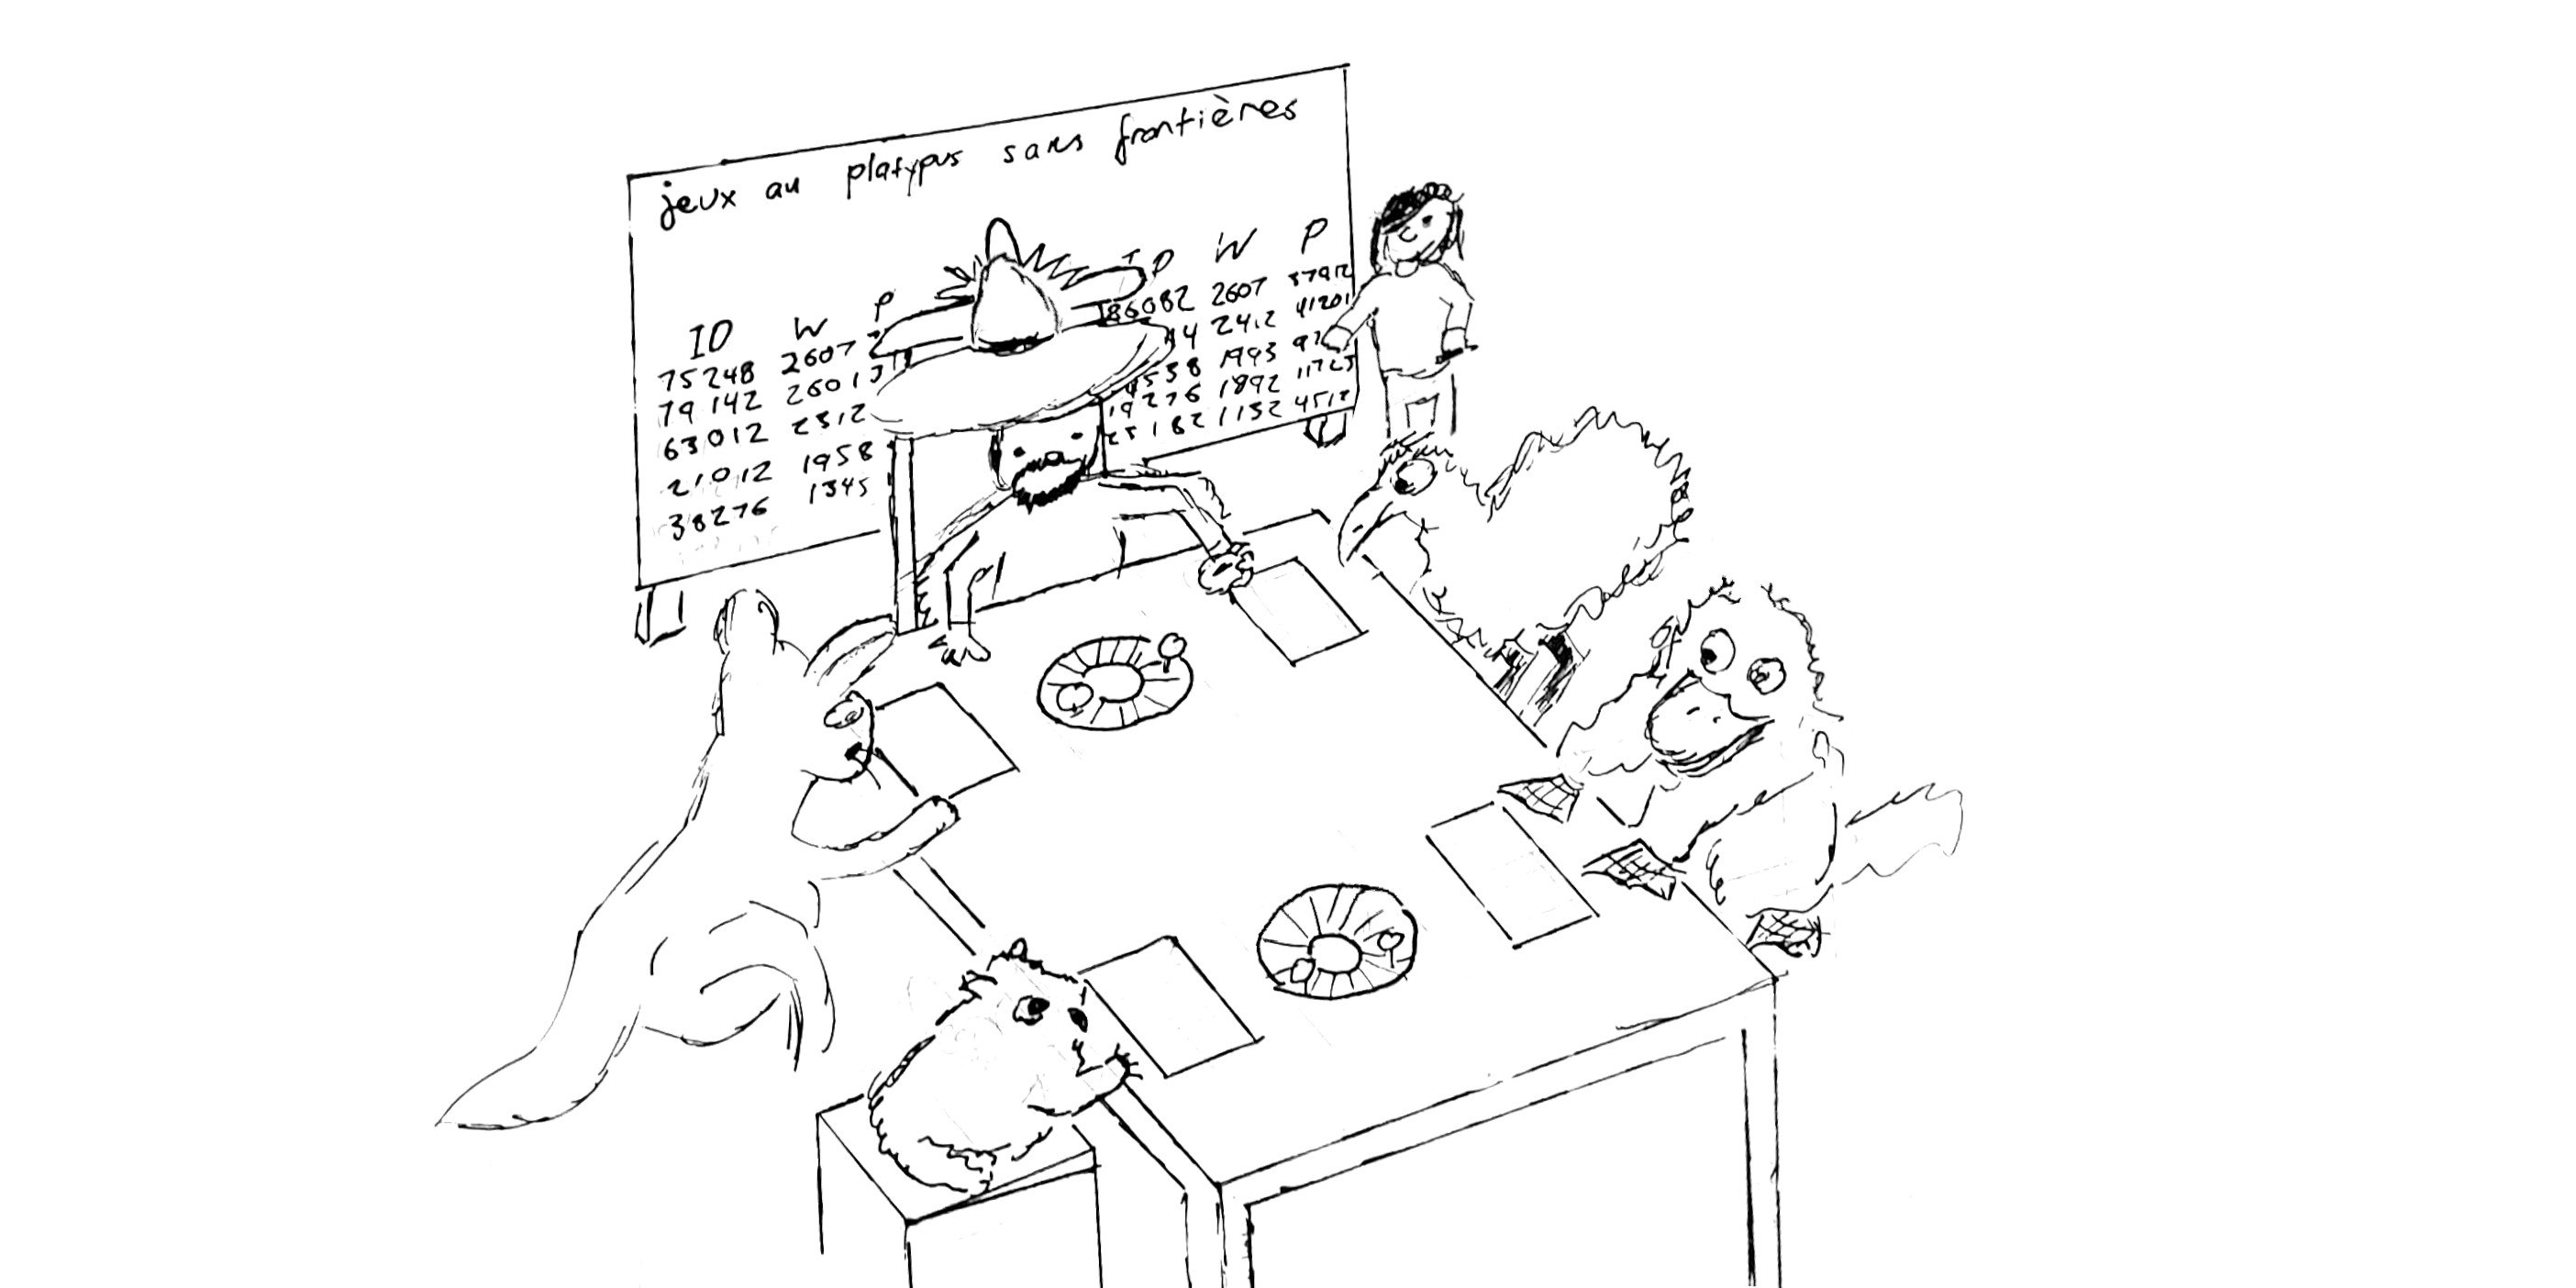
\includegraphics[width=\textwidth]{jeux-sans-frontieres.jpg}
  \btVFill
  {\huge\usebeamercolor[fg]{structure} Platypus Games Without Frontiers} \\
  \vspace{0.5em}
  Hayley Patton \hfill \today
  \vspace{0.5em}
\end{frame}

\begin{frame}
  \frametitle{The \emph{Platypus} game}

  \begin{center}
    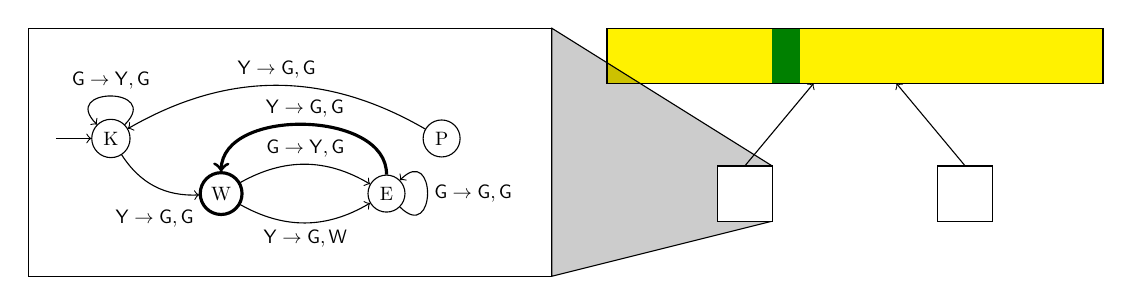
\begin{tikzpicture}[scale=0.7, every node/.style={scale=0.7}]
      % Match
      \fill[yellow] (9, 1) rectangle (18, 2);
      \fill[green!50!black] (12, 1) rectangle (12.5, 2);
      \draw (9, 1) rectangle (18, 2);
      % Machine cutout
      \draw[fill=black, fill opacity=0.2] (8, -2.5) -- (12, -1.5) -- (12, -0.5) -- (8, 2) -- (8, -2.5);
      \draw[fill=white] (11, -1.5) rectangle +(1, 1);
      \draw[->] (11.5, -0.5) -- (12.75, 1);
      \draw (15, -1.5) rectangle +(1, 1);
      \draw[->] (15.5, -0.5) -- (14.25, 1);
     
      % Internals
      \draw[fill=white] (-1.5, -2.5) rectangle (8, 2);
      \node[draw, circle] (P) at (6, 0) {P};
      \node[draw, circle, line width=0.4mm] (W) at (2, -1) {W};
      \node[draw, circle] (E) at (5, -1) {E};
      \node[draw, circle] (K) at (0, 0) {K};
      \draw[->] (-1, 0) to (K);
      \draw[->] (P) to[bend right] node[midway, above] {$\q{Y} \rightarrow \q{G}, \q{G}$} (K);
      \draw[->] (W) to[bend left] node[midway, above] {$\q{G} \rightarrow \q{Y}, \q{G}$} (E);
      \draw[->] (W) to[bend right] node[midway, below] {$\q{Y} \rightarrow \q{G}, \q{W}$} (E);
      \draw[->] (E) to[in=45, out=-45, looseness=5] node[midway, right] {$\q{G} \rightarrow \q{G}, \q{G}$} (E);
      \draw[->, line width=0.4mm] (E) to[bend right=90] node[midway, above] {$\q{Y} \rightarrow \q{G}, \q{G}$} (W);
      \draw[->] (K) to[in=135, out=45, looseness=5] node[midway, above] {$\q{G} \rightarrow \q{Y}, \q{G}$} (K);
      \draw[->] (K) to[bend right] node[midway, below=3mm] {$\q{Y} \rightarrow \q{G}, \q{G}$} (W);
     
    \end{tikzpicture}
  \end{center}

  \vspace{2em}
  268 million ($2^{28}$) machines, two players, 72 quadrillion ($2^{56}$) matches.
\end{frame}

\begin{frame}
  \frametitle{Optimisations}

  \begin{tabular}{lrrr}
    Single-threaded & 72 Pmatches & at 6 Mmatches/s & takes 381 years \\
    Equivalence detection & 2.9 Pmatches & & 15 years \\
    Multi-threaded & & 89 Mmatches/s & 1 year \\
    SIMD & & 436 Mmatches/s & 77 days \\
    GPU & & 1060 Mmatches/s & 32 days \\
    Cloud GPUs & & 3710 Mmatches/s & 9 days \\
    \hline
    Improvement & \small 25$\times$ & \small 618$\times$ & \small 15300$\times$ faster
  \end{tabular}
\end{frame}

\newcommand{\pcol}[1]{\color{cb1}{#1}}
\newcommand{\pani}[1]{\color{cb2}{#1}}
\newcommand{\pdir}[1]{\color{cb3}{#1}}

\begin{frame}
  \frametitle{Representing Platypus machines}
  \begin{center}
    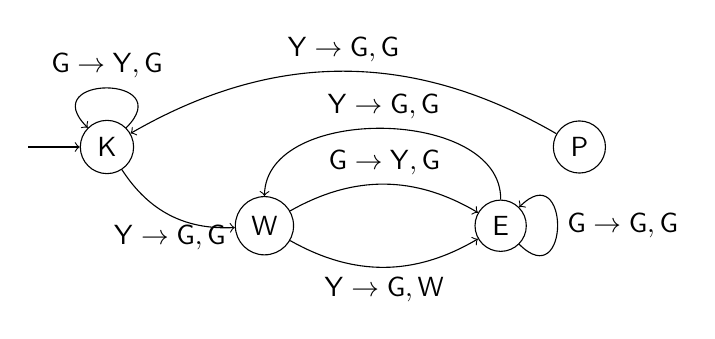
\begin{tikzpicture}
      \node[draw, circle] (P) at (6, 0) {\sffamily P};
      \node[draw, circle] (W) at (2, -1) {\sffamily W};
      \node[draw, circle] (E) at (5, -1) {\sffamily E};
      \node[draw, circle] (K) at (0, 0) {\sffamily K};
      \draw[->] (-1, 0) to (K);
      \draw[->] (P) to[bend right] node[midway, above] {$\q{Y} \rightarrow \q{G}, \q{G}$} (K);
      \draw[->] (W) to[bend left] node[midway, above] {$\q{G} \rightarrow \q{Y}, \q{G}$} (E);
      \draw[->] (W) to[bend right] node[midway, below] {$\q{Y} \rightarrow \q{G}, \q{W}$} (E);
      \draw[->] (E) to[in=45, out=-45, looseness=5] node[midway, right] {$\q{G} \rightarrow \q{G}, \q{G}$} (E);
      \draw[->] (E) to[bend right=90] node[midway, above] {$\q{Y} \rightarrow \q{G}, \q{G}$} (W);
      \draw[->] (K) to[in=135, out=45, looseness=5] node[midway, above] {$\q{G} \rightarrow \q{Y}, \q{G}$} (K);
      \draw[->] (K) to[bend right] node[midway, below] {$\q{Y} \rightarrow \q{G}, \q{G}$} (W);
    \end{tikzpicture}

    \begin{tabular}{rr|ccccccc}
      \hline
      From & Colour & Y & G & Y & G & Y & G & Y \\
      & Animal & K & K & E & E & W & W & P \\
      \hline
      To & Colour & \pcol{G} & \pcol{Y} & \pcol{G} & \pcol{G} & \pcol{G} & \pcol{Y} & \pcol{G} \\
      & Animal & \pani{W} & \pani{K} & \pani{W} & \pani{E} & \pani{E} & \pani{E} & \pani{K} \\
      & Direction & \pdir{G} & \pdir{G} & \pdir{G} & \pdir{G} & \pdir{W} & \pdir{G} & \pdir{G} \\
      \hline
      \\
      \multicolumn{2}{r}{Packed} &
      \texttt{\pdir{1}\pani{01}\pcol{0}} & \texttt{\pdir{1}\pani{11}\pcol{1}} & \texttt{\pdir{1}\pani{01}\pcol{0}} & \texttt{\pdir{1}\pani{10}\pcol{0}} & \texttt{\pdir{0}\pani{10}\pcol{0}} & \texttt{\pdir{1}\pani{10}\pcol{1}} & \texttt{\pdir{1}\pani{11}\pcol{0}}
    \end{tabular}
  \end{center}
\end{frame}

\begin{frame}
  \frametitle{Dead code elimination}
  \begin{center}
    \parbox{0.25\textwidth}{
      x $\leftarrow$ 1 \\
      \\
    }%
    \parbox{0.25\textwidth}{
      x $\leftarrow$ 1 \\
      \textbf{if} false \\
      \hspace*{1em} x $\leftarrow$ 2
    }%
    \parbox{0.25\textwidth}{
      x $\leftarrow$ 1 \\
      \textbf{if} 1 = 2 \\
      \hspace*{1em} x $\leftarrow$ 2
    }%
    \parbox{0.25\textwidth}{
      x $\leftarrow$ 1 \\
      \textbf{if} x = 2 \\
      \hspace*{1em} x $\leftarrow$ 2
    }
  \end{center}

  In all cases, x = 1.
\end{frame}

\begin{frame}
  \frametitle{Dead code elimination}
    \begin{center}
    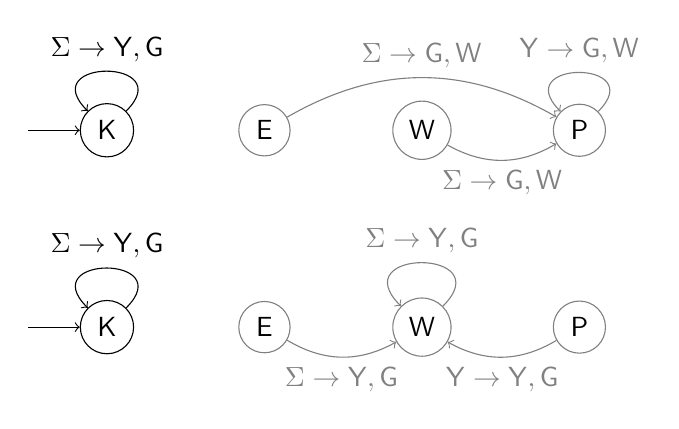
\begin{tikzpicture}
      \node[draw=gray, circle] (P1) at (6, 0) {\sffamily P};
      \node[draw=gray, circle] (W1) at (4, 0) {\sffamily W};
      \node[draw=gray, circle] (E1) at (2, 0) {\sffamily E};
      \node[draw, circle] (K1) at (0, 0) {\sffamily K};
      \draw[->] (-1, 0) to (K1);
      \draw[->, gray] (P1) to[in=135, out=45, looseness=5] node[midway, above] {$\q{Y} \rightarrow \q{G}, \q{W}$} (P1);
      \draw[->, gray] (W1) to[bend right] node[midway, below] {$\Sigma \rightarrow \q{G}, \q{W}$} (P1);
      \draw[->, gray] (E1) to[bend left] node[midway, above] {$\Sigma \rightarrow \q{G}, \q{W}$} (P1);
      \draw[->] (K1) to[in=135, out=45, looseness=5] node[midway, above] {$\Sigma \rightarrow \q{Y}, \q{G}$} (K1);
    
      \node[draw=gray, circle] (P2) at (6, -2.5) {\sffamily P};
      \node[draw=gray, circle] (W2) at (4, -2.5) {\sffamily W};
      \node[draw=gray, circle] (E2) at (2, -2.5) {\sffamily E};
      \node[draw, circle] (K2) at (0, -2.5) {\sffamily K};
      \draw[->] (-1, -2.5) to (K2);
      \draw[->, gray] (P2) to[bend left] node[midway, below] {$\q{Y} \rightarrow \q{Y}, \q{G}$} (W2);
      \draw[->, gray] (W2) to[in=135, out=45, looseness=5] node[midway, above] {$\Sigma \rightarrow \q{Y}, \q{G}$} (W2);
      \draw[->, gray] (E2) to[bend right] node[midway, below] {$\Sigma \rightarrow \q{Y}, \q{G}$} (W2);
      \draw[->] (K2) to[in=135, out=45, looseness=5] node[midway, above] {$\Sigma \rightarrow \q{Y}, \q{G}$} (K2);
    \end{tikzpicture}
  \end{center}

  40\% of machines remain after deduplicating by dead code elimination.
\end{frame}

\begin{frame}
  \frametitle{Renaming values}
  \begin{center}
    \parbox{0.33\textwidth}{
      x $\leftarrow$ 1 \\
    }%
    \parbox{0.33\textwidth}{
      y $\leftarrow$ 1 \\
      x $\leftarrow$ y
    }%
    \parbox{0.33\textwidth}{
      z $\leftarrow$ 1 \\
      x $\leftarrow$ z
    }
  \end{center}

  In all cases, x = 1.
\end{frame}

\begin{frame}
  \frametitle{Renaming states}
  \begin{center}
    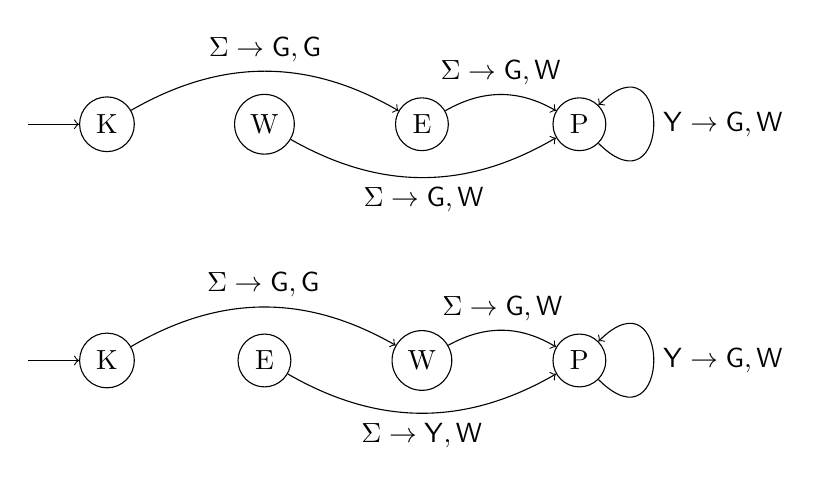
\begin{tikzpicture}
      \node[draw, circle] (P1) at (6, 0) {P};
      \node[draw, circle] (W1) at (4, 0) {W};
      \node[draw, circle] (E1) at (2, 0) {E};
      \node[draw, circle] (K1) at (0, 0) {K};
      \draw[->] (-1, 0) to (K1);
      \draw[->] (P1) to[in=45, out=-45, looseness=7] node[midway, right] {$\q{Y} \rightarrow \q{G}, \q{W}$} (P1);
      \draw[->] (W1) to[bend left] node[midway, above] {$\Sigma \rightarrow \q{G}, \q{W}$} (P1);
      \draw[->] (E1) to[bend right] node[midway, below] {$\Sigma \rightarrow \q{Y}, \q{W}$} (P1);
      \draw[->] (K1) to[bend left] node[midway, above] {$\Sigma \rightarrow \q{G}, \q{G}$} (W1);
      
      \node[draw, circle] (P2) at (6, 3) {P};
      \node[draw, circle] (W2) at (2, 3) {W};
      \node[draw, circle] (E2) at (4, 3) {E};
      \node[draw, circle] (K2) at (0, 3) {K};
      \draw[->] (-1, 3) to (K2);
      \draw[->] (P2) to[in=45, out=-45, looseness=7] node[midway, right] {$\q{Y} \rightarrow \q{G}, \q{W}$} (P2);
      \draw[->] (W2) to[bend right] node[midway, below] {$\Sigma \rightarrow \q{G}, \q{W}$} (P2);
      \draw[->] (E2) to[bend left] node[midway, above] {$\Sigma \rightarrow \q{G}, \q{W}$} (P2);
      \draw[->] (K2) to[bend left] node[midway, above] {$\Sigma \rightarrow \q{G}, \q{G}$} (E2);
    \end{tikzpicture}
  \end{center}

  20\% of machines remain after deduplicating by renaming (and DCE).

  We play every machine against every other, so this is a $5^2 = 25\times$ reduction in matches.
\end{frame}

\begin{frame}
  \frametitle{Multithreading}
  Parallelising the games themselves is boring, because games are independent.

  Communicating all the results is difficult, because games are faster than synchronisation.

  \pause

  \begin{itemize}
  \item Using a shared table requires atomic updates, which have substantial latency:
    50\,ns on a 12-core processor, 115\,ns on a 64-core.
  \item Using tables local to each thread requires a lot of memory and a lot of memory
    bandwidth.
  \end{itemize}

  Hybrids are possible:

  \begin{itemize}
  \item Have local chunks which are periodically synchronised with the
    shared table. More complex, with a more complex cost model.
  \item Simpler is to have a thread process every match involving a machine,
    which ensures mutual exclusion without atomics, but this doubles the
    work needed.
  \end{itemize}
\end{frame}

\begin{frame}
  \frametitle{Single instruction, multiple data}

  Modern processors have \emph{vector extensions} which can perform the same
  operation/instruction on multiple data at once.

  AVX2 provides 256-bit vectors, and almost all Platypus game data fits in
  32-bit values, so we can run 8 games simultaneously in each vector \emph{lane}.

  Platypus games have variable lengths, which complicates scheduling.
\end{frame}

\newcommand{\game}[4]{
  \draw[fill=white] (#1, #2) rectangle +(#3, 0.5);
  \node at (#1 + 0.25, #2 + 0.25) {#4};
}

\begin{frame}
  \frametitle{Scheduling games}

  We could wait for all games to finish, but this leaves gaps in the schedule.
  
  
\begin{tikzpicture}
    \draw[fill=black!20!white] (0, 0) rectangle (12, 2);
    \game{0}{1.5}{1}{1}
    \game{0}{1}{1}{2}
    \game{0}{0.5}{6}{3}
    \game{0}{0}{1}{4}
    \game{6}{1.5}{6}{5}
    \game{6}{1}{1}{6}
    \game{6}{0.5}{1}{7}
    \game{6}{0}{1}{8}
  \end{tikzpicture}

  Gaps cost about 15\% to 32\% in throughput. \pause Better would be:
  
  
\begin{tikzpicture}
    \draw[fill=black!20!white] (0, 0) rectangle (7, 2);
    \game{0}{1.5}{1}{1}
    \game{0}{1}{1}{2}
    \game{0}{0.5}{6}{3}
    \game{0}{0}{1}{4}
    \game{1}{1.5}{6}{5}
    \game{1}{1}{1}{6}
    \game{6}{0.5}{1}{7}
    \game{1}{0}{1}{8}
  \end{tikzpicture}
  
  The latter requires an \emph{expand} operation, which must be
  implemented by hand (and I fixed a compiler bug while doing so).
\end{frame}

\begin{frame}
  \frametitle{Cloud computing}

  General purpose computing on GPUs works quite well for
  Platypus games due to sheer parallelism.
  
  But I don't have the most amazing of GPUs in my desktop, and
  cloud computing hosts have better GPUs. I also rented two
  GPUs to get results faster, which involves distributed
  computing.
\end{frame}

\begin{frame}
  \frametitle{Distributed computing}
  \begin{columns}
    \begin{column}{0.5\textwidth}
      A distributed model provides some fault tolerance
      and flexibility in configuring the resources used to run
      the Platypus tournament. A server allocates work to
      clients and records the results achieved by each machine.

       AWS offers multi-GPU instances, but only with
       lots of CPU cores and memory which I don't need;
       using multiple single-GPU instances is more cost
       effective.
    \end{column}
    \begin{column}{0.5\textwidth}
      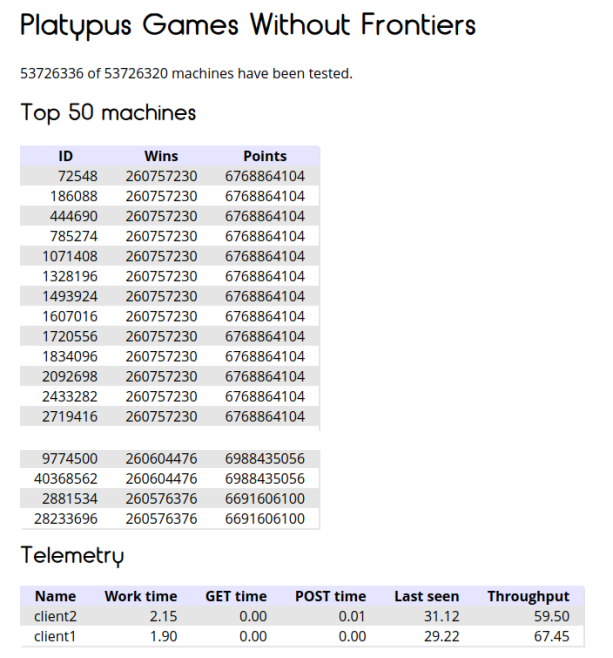
\includegraphics[width=\textwidth]{control.png}
    \end{column}
  \end{columns}
\end{frame}

\begin{frame}
  \frametitle{The winners}
  \begin{center}
    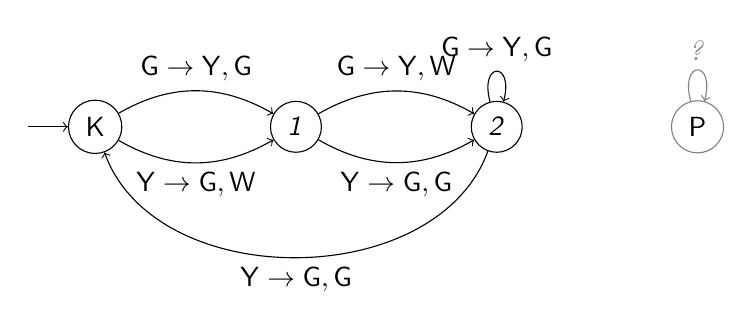
\begin{tikzpicture}[scale=0.85]
      \node[draw, circle] (K) at (0, 0) {\sffamily K};
      \node[draw, circle] (W) at (3, 0) {\sffamily \emph{1}};
      \node[draw, circle] (E) at (6, 0) {\sffamily \emph{2}};
      \node[draw=gray, circle] (P) at (9, 0) {\sffamily P};
      \draw[->] (-1, 0) to (K);
      \draw[->] (K) to[out=-30, in=-150] node[midway, below] {$\q{Y} \rightarrow \q{G}, \q{\pdir{W}}$} (W);
      \draw[->] (K) to[out=30, in=150] node[midway, above] {$\q{G} \rightarrow \q{Y}, \q{\pdir{G}}$} (W);
      \draw[->] (E) to[out=-110, in=-70] node[midway, below] {$\q{Y} \rightarrow \q{G}, \q{\pdir{G}}$} (K);
      \draw[->] (E) to[loop above] node[midway, above] {$\q{G} \rightarrow \q{Y}, \q{\pdir{G}}$} (E);
      \draw[->] (W) to[out=-30, in=-150] node[midway, below] {$\q{Y} \rightarrow \q{G}, \q{\pdir{G}}$} (E);
      \draw[->] (W) to[out=30, in=150] node[midway, above] {$\q{G} \rightarrow \q{Y}, \q{\pdir{W}}$} (E);
      \draw[->, gray] (P) to[loop above] node[midway, above] {\emph{?}} (P);
    \end{tikzpicture}
    
    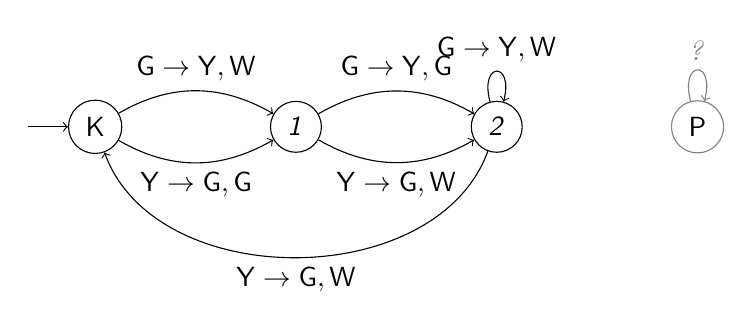
\begin{tikzpicture}[scale=0.85]
      \node[draw, circle] (K) at (0, 0) {\sffamily K};
      \node[draw, circle] (W) at (3, 0) {\sffamily \emph{1}};
      \node[draw, circle] (E) at (6, 0) {\sffamily \emph{2}};
      \node[draw=gray, circle] (P) at (9, 0) {\sffamily P};
      \draw[->] (-1, 0) to (K);
      \draw[->] (K) to[out=-30, in=-150] node[midway, below] {$\q{Y} \rightarrow \q{G}, \q{\pdir{G}}$} (W);
      \draw[->] (K) to[out=30, in=150] node[midway, above] {$\q{G} \rightarrow \q{Y}, \q{\pdir{W}}$} (W);
      \draw[->] (E) to[out=-110, in=-70] node[midway, below] {$\q{Y} \rightarrow \q{G}, \q{\pdir{W}}$} (K);
      \draw[->] (E) to[loop above] node[midway, above] {$\q{G} \rightarrow \q{Y}, \q{\pdir{W}}$} (E);
      \draw[->] (W) to[out=-30, in=-150] node[midway, below] {$\q{Y} \rightarrow \q{G}, \q{\pdir{W}}$} (E);
      \draw[->] (W) to[out=30, in=150] node[midway, above] {$\q{G} \rightarrow \q{Y}, \q{\pdir{G}}$} (E);
      \draw[->, gray] (P) to[loop above] node[midway, above] {\emph{?}} (P);
    \end{tikzpicture}
  \end{center}
\end{frame}

\begin{frame}
  \frametitle{What's next?}
  \begin{itemize}
  \item Analyse the results of the full Platypus tournament.
  \item Apply the methodology to variations of the Platypus game.
  \item Use the results to find the accuracy of other competition structures (e.g. knockout).
  \end{itemize}
\end{frame}
\end{document}

% Local Variables:
% TeX-engine: xetex
% End:
